\documentclass[a4paper,12pt]{article}
\setlength{\parskip}{0.5pt}%
\setlength{\parindent}{20pt}%

%preamble: style and/or packages
\author{Margaret Murakami}
\title{PhD research proposal}
\date{January 2023}

%\usepackage{package}

\usepackage{hyperref}
\usepackage{titlesec}
\setcounter{secnumdepth}{3}
\usepackage{enumitem}
\usepackage{varwidth}
\usepackage{tasks}

\usepackage{graphicx}
\usepackage{siunitx}

%colors, boxes
\usepackage[dvipsnames]{xcolor}
\usepackage[most]{tcolorbox}
\tcbuselibrary{fitting}

\definecolor{columbiablue}{rgb}{0.61, 0.87, 1.0}
\definecolor{mossgreen}{rgb}{0.68, 0.87, 0.68}


% Use biblatex instead of natbib
% \usepackage[style=authoryear]{biblatex} % Set citation style to author-year
% \addbibresource{references.bib} % Specify your .bib file here

\usepackage[super,sort&compress,comma]{natbib}
%\usepackage[round,authoryear]{natbib}
%\usepackage[authoryear]{natbib}
\bibliographystyle{naturemag}

%indent first line
\usepackage{indentfirst}
\setlength{\parindent}{30pt}

%captions
\usepackage[font=footnotesize,labelfont={bf,it}, textfont=it]{caption}
\usepackage[labelsep=period]{caption}

%landscape pages
\usepackage{pdflscape}
\usepackage{fancyhdr} 

%page number at bottom in landscape 
\fancypagestyle{mylandscape}{
\fancyhf{} %Clears the header/footer
\fancyfoot{% Footer
\makebox[\textwidth][r]{% Right
  \rlap{\hspace{.75cm}% Push out of margin by \footskip
    \smash{% Remove vertical height
      \raisebox{4.87in}{% Raise vertically
        \rotatebox{90}{\thepage}}}}}}% Rotate counter-clockwise
\renewcommand{\headrulewidth}{0pt}% No header rule
\renewcommand{\footrulewidth}{0pt}% No footer rule
}

%temporarily disable superscript
\DeclareRobustCommand*{\citen}[1]{%
  \begingroup
    \romannumeral-`\x % remove space at the beginning of \setcitestyle
    \setcitestyle{numbers}%
    \cite{#1}%
  \endgroup   
}



\begin{document}
	
	% cover page
	\begin{center}
	\thispagestyle{empty}
		\begin{LARGE}
		\textbf{Arctic Ocean Water Mass Transformation (WMT) in the Arctic Subpolar gyre sTate Estimate (ASTE): Budget Analysis in Temperature-Salinity Space} \\[1 cm] \vfill
		\end{LARGE}
			
			
		\begin{Large}
			PhD research proposal \\ [1 cm]\vfill
			Margaret Murakami \\
			\href{mailto:<email>}{mmurakami@utexas.edu} \\[1 cm]\vfill
			
			
			November, 2024\\[1 cm]\vfill

                \textbf{Examining Committee}: Dr. Patrick Heimbach (supervisor), Dr. Peter Flaig (chair), Dr. Geeta Persad, Dr. Marc Hesse, Dr. Ann Ruth (Ruthie) Halberstadt \\[1 cm]\vfill
			
            % Choose between bnw or rgb logos
            \begin{center}
                \begin{minipage}{0.45\textwidth}
                    \centering
                    
\includegraphics[width=\linewidth]{../figures/CMYK_formal_Oden_ICES.pdf}
                    % Caption or label if necessary
                \end{minipage}%
                \hfill
                \begin{minipage}{0.45\textwidth}
                    \centering
                    
\includegraphics[width=\linewidth]{../figures/jsg_formal_fullColor.png}
                    % Caption or label if necessary
                \end{minipage}
            \end{center}
            
			
		\end{Large}
	\end{center}
	
	% document begins
	\newpage
	%%table of contents 
	{\setlength\parskip{\fill}
		\tableofcontents
	}

    %you can start a new page anytime with \newpage
	\newpage

        % Objective
        \section*{Objective}
        \addcontentsline{toc}{section}{\protect\numberline{}Objective}
        The overarching goal of the proposed work is to investigate the influence of the changing climate on the stratification and circulation of the Arctic Ocean using the Arctic Subpolar gyre sTate Estimate (ASTE).
	
	%Abstract
	%\section*{Abstract}
	%\addcontentsline{toc}{section}{\protect\numberline{}Abstract}
		
	%%Introduction
    %\newpage
	\section{Description of the Research Project}
 
	\subsection{Goals of the Research}
        % introduction - what has the Arctic been like the last decades
        The Arctic climate and the climatology of the Arctic Ocean have undergone rapid changes in recent decades. These include rising near-surface air temperatures \cite{Screen2010}, shifts in river runoff and glacial discharge \cite{Proshutinsky2020,Nummelin2015}, an increased influx of freshwater through the Bering Strait \cite{Woodgate2018,Woodgate2021}, and enhanced heat transport from the Atlantic, which can propagate into the Barents Sea \cite{Hakkinen2009}. Such changes in heat and salt forcing have substantial implications on the stratification of the Arctic Ocean itself. For example, changes to wind-driven mixing, ice melt, and runoff have caused an accumulation of freshwater in the Beaufort Gyre \cite{Proshutinsky2002,Proshutinsky2020,Giles2012}. Notably, the Arctic has also experienced a rapid decline in multi-year sea ice \cite{Perovich2009}, with implications for the surface heat forcing of the Arctic Ocean. Many of these changes are considered to feed positive feedback loops for sea ice: decreased sea ice extent is linked to decreases in surface albedo and increased shortwave absorption \cite{Timmermans2018,Pistone2019}, increased heat flux through the Fram and Barents Straits \cite{Lind2018,Wang2020}, and allows for ventilation of the Atlantic Water to the Arctic Ocean interior \cite{Polyakov2017}.

        % stratification of the Arctic as an example
        Unlike most of the global oceans which are stratified by temperature, the Arctic Ocean is characterized by a cold, fresh surface layer (Arctic Water) overlying a warmer, saltier Atlantic Water (AW) layer \cite{Carmack2007}. This stratification by salinity is crucial in keeping AW heat at depth, as well as maintaining sea ice cover and ventilating the Arctic Ocean \cite{Wang2020}.

        % some more on the Arctic - what is predicted to happen
        Arctic amplification and impact of AW on sea ice
        
        % Barents Sea - why do we care about it and how is it concentrating heat
        Arctic warming is non-uniform and is amplified in the Barents and Kara Seas, which feature the strongest decline in winter sea ice concentration and some of the most rapid warming in the entire Arctic \cite{Screen2010}.
        as well as changes to heat transport to the Arctic Ocean from the subpolar North Atlantic \cite{Wang2019}, the prin ...
        Talk about Lind et. al 2018 and Wang et. al 2019.
        Ocean warming is not limited to the Arctic Ocean, and warming in the subpolar North Atlantic can have downstream impacts on the Barents Sea 

        % goals/aims
        The aim of this study is quantify how the observed warming of the Arctic Ocean can be attributed to the change in sea ice extent, area and concentration, and that these changes allow for advection of Atlantic Water to the central Arctic. The changing role of the Barents Sea is an important component of the Arctic heat budget \cite{Arthun2016}, and can be quantified by budget analysis. We anticipate the respective role of the sea ice as a surface process on the buoyancy changes of the Barents Sea and the Arctic to explain the observed temperatures and salinity changes in this region. Furthermore, because budget analysis has not yet been used in coordination with water mass transformation (WMT), it has not yet been possible to quantify the respective role of horizontal advection as compared with vertical diffusion and other mechanisms in the atmosphere and ocean as impacts on ocean buoyancy.

        % Overarching goal
        The overarching goal of this project is to resolve the relative contribution of the changes in surface forcing with forcing by transport from lower latitudes. Budgeted diagnostics resolved using ASTE will be used to diagnose the advection of Atlantic Water into the Arctic and resolve its heat loss in the Arctic Ocean, as well as its impact on the changing stratification of the Arctic. By using these diagnostics to reliably resolve and pinpoint, the most important processes to the changing climatology of the Barents Sea and the Arctic, we will resolve gaps in the understanding of these regions, paving the way for future climate research.

    
    %\newpage
    \subsection{State of the art}
    % one paragraph summarizing past WMT to the Arctic (Walin, Hieronymus, etc)
    The stratification of the world's oceans is determined by density, a product of salinity \emph{S} and temperature \emph{T}. The distributions of \emph{S} and temperature \emph{T} depend on several factors, including atmospheric fluxes, large-scale circulation, and vertical processes. In particular, the sea ice formation and distribution can play and important role on \emph{S} changes at the ocean surface, causing both freshening and salting of the water column, during the seasonal cycle of ice formation. One approach to studying buoyancy changes in the global ocean has been to translate the geographic distribution of ocean volume to explicitly defined \emph{T} and \emph{S} as coordinates. First used to study flow across isohaline \cite{Walin_1977} or isothermal \cite{Walin1982} surfaces, analysis of volume transport in \emph{T}-\emph{S} space has been applied in several subsequent studies in the North Atlantic \cite{Speer1993}, across gateways to the Arctic \cite{Rudels2008}, and across the pan-Arctic domain \cite{Pemberton2015} to study regional WMT. A framework to formulate volume, heat and salinity budgets has also been developed in which a change in water buoyancy is shown as a vector in \emph{T}-\emph{S} coordinates \cite{Speer1993,Hieronymus2014}. An example of this is shown in Figure~\ref{fig:groeskamp}, where fluid volumes can be displaced by heat fluxes in the \emph{T} direction and by salt fluxes in the \emph{S} direction. Performing analyses in \emph{T}-\emph{S} space–rather than geographic space–allows for the quantification of dominant salinity or temperature driven processes in transforming distinct water masses.

    %figure template
    \begin{figure}[ht]
    \centerline{
    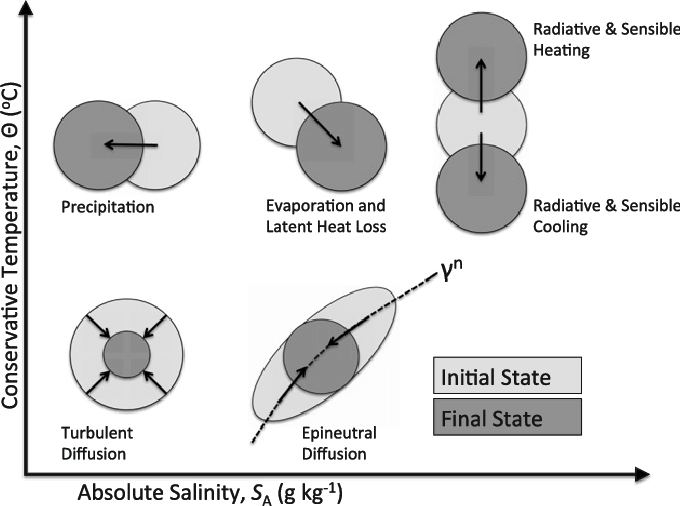
\includegraphics[width=\linewidth]{../figures/groeskamp_schematic.png}
    }
    \caption{Several possible modifications to \emph{T} and \emph{S} in the ocean are possible. This schematic shows how fluid can be displaced through WMT. Arrows represent WMT, shaded regions depict volume distribution in \emph{T}--\emph{S} space, and $\gamma_n$ represents a surface of neutral density \cite{Groeskamp2014}}
    \label{fig:groeskamp}
    \end{figure}
   

    % Arctic and Subpolar North Atlantic and Barents Sea
    A few primary water masses--defined by discrete sets of T and S values--interact in the Arctic Ocean: cold, fresh Arctic Water and salty, warm Atlantic Water (AW). Pacific water, which is relatively fresh and warm, also plays an important role in the blending of water properties in the Western Arctic, particularly through the Bering Strait inflow \cite{Haine2015}. An important gateway regulating this exchange of water masses is the Barents Sea Opening (BSO), across which the northward advection of AW provides heat and salt to the Barents Sea. The Barents Sea has been considered a kind of buffer zone between the Atlantic Ocean and the Arctic.

    However, the sea ice decline in this region has been faster than anticipated with climate models (SOURCE) and its climatology is changing radidly. Thus, establishing detailed records of its Atlantification is of the utmost importance both for regional studies and to understand the implications on the internal Arctic
    
    % Eastern Arctic studies
    Beyond the Barents Sea, there is particular interest on changes to the heat content of the mixed layer in the Eastern Arctic continental shelf \cite{Schulz2022}. \cite{Polyakov2017}

    % discussion of this and other model studies; like Pemberton
    Developments in the \emph{T}--\emph{S} framework have been important to quantify the most dominant fluxes on ocean buoyancy in the Arctic, helping both to understand the past Arctic Ocean as well as predicting future stratification changes \cite{Pemberton2015}. However, budget analysis remains technically difficult, leaving uncomfortably large residuals in WMT studies, and making it difficult to analyze small-scale ocean processes beyond the most dominating terms. Thus, there still exist many uncertainties surrounding the role of specific processes in the Arctic responsible for the observed changes in heat and salt transport over the last decades. Closed budgets of heat, salt, and mass on the grid scale enable novel robust assessment of the relative roles of surface, advective and diffusive fluxes for the modification of water masses. Using budget analysis, we begin to unpack recent buoyancy changes in more detail, pinpointing exactly which processes are most responsible for the changing \emph{T}--\emph{S} distribution in various basins of the Arctic.

    % Adjoint sensitivity studies
    The adjoint method can be a useful tool to study the attribution of specific changes to forcing terms \cite{Heimbach2011,Pillar2016,Smith2019,Nguyen2020}.
    
    %\vspace*{5mm}

    %Objective and research questions
    %\newpage
    \section{Research Project}
    One primary research question guides our work: How do sea ice, atmospheric forcing, and the ocean influence the changing regimes of the Arctic Ocean? Understanding the precise impacts of various diagnostics is vital to understanding past warming and freshening of the Arctic Ocean. The ability to fully represent surface processes and advection as impacts on ocean buoyancy provides new insights on the impact of climate change on the Arctic. Furthermore, we hypothesize study of the Arctic Ocean in the Water Mass Transformation (WMT) will reveal similar regime shifts across different Arctic basins, despite regional differences. We address this issue with three primary work packages.

    \subsection{Existing and Derived Data Products}\label{ASTE}
    % ASTE and what we can say about it
    We utilize the Arctic Subpolar gyre sTate Estimate (ASTE), the coupled ocean-sea ice model that is an advanced version of the Massachusetts Institute of Technology general circulation model (MITgcm). 

    ASTE is based on the medium resolution LLC-270 grid, which features a nominal grid spacing of $1/3^\circ$ over the period 2002--2017. The model is constrained to $10^9$ satellite and in situ observations.

    % Data we are using and why, talk about the budgets
    For projects 1--2, we use monthly mean output for the model period from 2002--2017. The budgets are created using...

    For project 3, we will use the adjoint method to perform our analysis of the ocean.
    % write

    \subsection{Projects}
    Here I propose to perform a comprehensive study of the controls on Arctic WMT using budget analysis in ASTE with a focus on Atlantification and heat transport. This work will aim to address open questions within the field of Arctic Oceanography:

    \begin{enumerate}
        \item Q1: What drives the rapid warming and salinification of the Barents Sea? What forcing terms are most important to understand its rapid change and what implications does this have for the Arctic Ocean?
        \item Q2: How is Atlantification changing the climatology of the eastern Arctic? How can we relate changing sea ice to the inflow of heat through the Eastern Arctic? How can we investigate the causes of Atlantification by examining the heat loss of AW?
        \item Q3: What controls anomalies in the stratification of the Eastern Arctic? What are the most substantial drivers of changes in buoyancy and on what timescales are these important?
    \end{enumerate}

    To answer these questions, we propose three hypotheses, which will guide the three projects we approach and serve as a basis to test our analyses:

    \begin{enumerate}
        \item H1: Budget analysis will show that rapid warming and salinification of the Barents Sea are driven by changes to surface forcing, including by sea ice retreat. While advection plays a role in WMT, the enhanced role for surface processes has resulted in the net formation of warmer, saltier water masses.
        \item H2: In the Eastern Arctic, intensified Atlantic heat transport along the Eastern Siberian continental shelf, driven by vertical mixing, is the primary factor in reducing stratification and contributing to Atlantification. We hypothesize that the impact of sea ice retreat is differentiable from the impact of wind forcing, yet both allow this vertical mixing to increase, allowing heat to enter the mixed layer.
        \item H3: Adjoint reconstruction allows us to gain further insights into the changes to the mixed layer from results of Project 1 and 2. We hypothesize that by using a physics-based approach in the Eastern Arctic, we can identify the timescales on which salt dynamics in the mixed layer can be attributed to surface forcing.
    \end{enumerate}

    \subsubsection{Project 1: the Barents Sea in a changing climate: a key benefit of budget analysis}
    
    \begin{tcolorbox}[minipage,colback=Goldenrod,arc=10pt,outer arc=10pt]
    \centering
    \textbf{Method:}	\emph{Budget analaysis for early and late years in ASTE}\label{sec1_1}
    \end{tcolorbox}
    % BROAD AIM: look at heat transport and causes of convergence in the barents sea
    The aim of the first project is to apply budget analysis within a simulation of ASTE \cite{Nguyen2021} to examine WMT in the Barents Sea. As described in section \ref{ASTE}, budget analysis will be performed in the Barents Sea using monthly outputs of the model. The focus of this paper will be on heat loss within the Barents Sea with a particular focus on the convergence of volume in warmer, saltier water masses in \emph{T}--\emph{S} space. For this project, we will use the ASTE
    
    % the breakdown of the budget
    Budget analysis from the model is calculated from the ocean state, recorded at the beginning of each month in the time period from 2002--2017. For eeach grid cell, the forcing terms on heat, salt and mass are budgeted using the conservation laws such that the sum of various diagnostics is equal to zero in each grid cell. However, further breakdown of the surface terms -- in particular the atmospheric and ocean influences on sea ice -- may require additional diagnostics from the ASTE Release 1 \cite{Nguyen2021}. This will be an opportunity for modification of the budgeting scripts and a comparison of the t...

    % what we are using and what we aim to solve
    Initial simulations will span two, five-year periods: 2003--2007 and 2013--2017. The purpose of this comparison is to provide a broad overview of the two periods and to demonstrate the changing terms in ASTE in early and late years of the model simulation. For these two periods, we aim to observe the impacts of changing sea ice and surface forcing. This avoids the first year immediately after the spin-up. 


    % how we are going to break down the budget

    \begin{tcolorbox}[minipage,colback=Goldenrod,arc=10pt,outer arc=10pt]
    \centering
    \textbf{Expected Results:}	\emph{A key role for surface forcing}\label{sec1_2}
    \end{tcolorbox}
    % what is the goal
    Through the WMT framework in ASTE, a closer examination of the long-term forcings in the Barents Sea will be completed. This tasks aims to quantify any long-term tendencies in the Barents Sea, and determine governing forces on long-term heat and salt changes from the model output.

    % how are we going to look closer at the two time periods

    \subsubsection{Project 2: Connecting the Atlantic Sector to the heat transport of the Eastern Arctic}
    
    \begin{tcolorbox}[minipage,colback=columbiablue,arc=10pt,outer arc=10pt]
    \centering
    \textbf{Method:}	\emph{Applied budget analysis with a focus on surface forcing}\label{sec2_1}
    \end{tcolorbox}
    % BROAD AIM: changes to the mixed layer as a result of sea ice/winds
    % how do we build on the results of the previous paper
    The Barents Sea analysis will demonstrate how Atlantification is changing the Atlantic sector. This provides information on the impact of sea ice loss on Atlantic inflow, however it does not tell us about the changes to stratification in the central Arctic Ocean, where the largest sea ice extents are. The primary goal of this WP is to leverage \emph{T}--\emph{S} analysis to better understand how AW influences the internal Arctic. Again, a key advantage of ASTE is its use of closed budgets on the grid scale, allowing our results to provide more detailed insights into smaller-scale processes, rather than focusing solely on the dominant forcing terms typically provided by other ocean general circulation models (OGCMs).

    % central question
    The central question this WP seeks to address is: how are shifting temperature and salinity trends propagating through the internal Arctic? By tracking tendencies influencing heat in various basins of the Arctic--from the Atlantic sector to the Western Arctic--we will evaluate how various terms are changing the Arctic Ocean water mass distributions.

    TWO FOCII OF THE ANALYSIS: the seasonal cycle and the relationship between surface forcing and internal processes

    % expected results
    The results from this task will build upon long-term tendencies identified in WP 1, focusing on the evolving diapycnal mixing and stratification changes over the ASTE period. We will follow the path of Atlantic Water around the Arctic, expanding from the Barents Sea to discuss heat transport in the Greenland, Iceland, and Norwegian Seas (GINS). Furthermore, it will address how tendencies change as Atlantic Water circulates the Arctic and is modified in important basins including the Nansen, Amundsen, Makarov, and Canada Basin. This comprehensive analysis will describe the evolving climatology of the Arctic Ocean.
    
    \begin{tcolorbox}[minipage,colback=columbiablue,arc=10pt,outer arc=10pt]
    \centering
    \textbf{Task 2.2}	\emph{Investigate stratification how stratification changes are explained by sea ice diagnostics}\label{sec2_2}
    \end{tcolorbox}
    % what do we anticipate looking closer at
    As rapid declines in Arctic sea ice extent continue, surface forcing on the Atlantic Ocean is undergoing substantial changes. We aim to address: how are these surface changes influencing internal stratification of the Arctic, and what consequences does this have for advection of AW into the Arctic?

    % how will we investigate this
    Building on the broad analysis in section \ref{sec2_1}, this task will look more closely at sea ice dynamics, and specifically how the changing distribution of sea ice alters internal stratification and diapycnal mixing. Because sea ice is known to maintain the stratification of the ocean, this task aims to quantify how its changes alter other tendencies, including by advection or internal mixing, and what implications this has for freshwater and heat storage. In this task, we aim to use the budget for the sea ice in detail, studying how the atmosphere-ice and ice-ocean interactions alter the changes in \emph{T}--\emph{S} distribution.


    % anticipated results
    This analysis will insight into the connection between sea ice and AW transport.

    
    \begin{tcolorbox}[minipage,colback=columbiablue,arc=10pt,outer arc=10pt]
    \centering
    \textbf{Task 2.3}	\emph{Inter-model comparison with other studies?? Model development with ASTE??}\label{sec2_3}
    \end{tcolorbox}
    % compare to Pemberton
    Of interest to the scientific community is not only to use our results to compare with 
    
    3-4 pages on a more pan-Arctic study, this will include comparing our work to Pemberton and other models.

    \subsubsection{Project 3: Adjoint sensitivity in the Eastern Arctic}

    \begin{tcolorbox}[minipage,colback=mossgreen,arc=10pt,outer arc=10pt]
    \centering
    \textbf{Task 3.1} \emph{Dimensionality reduction and clustering in ASTE}
    \end{tcolorbox}\label{sec3_1}

    % BROAD AIM: adjoint sensitivity study focused on mixed layer salt

    % how can clustering be added
    Using the results from the previous two work packages, WP 3 will synthesize ideas to determine the connectivity and importance of various regimes. A specific target of our research will be the 2012 sea ice minimum, with an explicit goal to determine the response of the ocean to such changes. This will be 

    % what we will do - similar to Maite Sonnewald
    Using a process of 

    \begin{tcolorbox}[minipage,colback=mossgreen,arc=10pt,outer arc=10pt]
    \centering
    \textbf{Task 3.2} \emph{Analyze causes of convergence through clustered analysis}\label{sec3_2}
    \end{tcolorbox}

    % what are we interested in
    The aimed analysis of the clusters will be two-fold. Of importance to the scientific community is not only which regions or regimes are most impacted by the changing climate and why, but also which regimes feature the most long-term accumulation of heat or salt.

    % importance of accumulation in ocean models
    Beyond the buoyancy transformations of the water masses in the ocean, predicting accumulation of heat or salt is of particular interest to the oceanographic community. To access the impacts of various ocean processes on these these dynamics, it 

    % return to the overarching goal for the project
    WP 3 will also return to the hypothesis proposed for the project. By demonstrating that ocean basins are dynamically similar, we prove that understanding causes of WMT is vital to understanding observed changes to heat transport and sea ice, leading to the completion of this research project. Further identifying dynamical regions which highlight the relationships between horizontal advection, vertical diffusion, and surface forcing on the heat gain of the Arctic will confirm that each of these terms are related and each are key considerations in modeling of the Arctic.

    %Methods
    \newpage
    \section{Outcomes and Significance of the Proposed Work}
	
     
    
    % you can find the template for this gantt chart in /figures/gantt_template.pptx, convert it to pdf and then to png to upload it on the document

    %example of a temporarily horizontal page
    \section{Work plan}
    The Ph.D. program was started in Fall 2023. Anticipating the defense in Spring 2028, the degree timeline will resemble the following:

    \begin{enumerate}
        \item \textbf{Coursework, literature review, and preparing budgeting scripts:} Fall 2023 -- Spring 2024

        Deliverable: Python scripts to perform budget analysis in ASTE, 
        
        \item \textbf{WP1:} Spring 2024 -- Fall 2024
        
        Deliverable: publication on the configuration of budget analysis tools to study changes to the Barents Sea, with a focus on the impacts of changing sea ice
        
        \item \textbf{WP2:} Spring 2025 -- Fall 2025

        Deliverable: publication synthesizing the influence of internal mixing versus surface forcing on the changes to the Arctic Ocean heat transport 

        \item \textbf{WP3:} Spring 2026 -- Fall 2026

        Deliverable: publication using clustering to synthesize the changing regimes of the Arctic Ocean basins

        \item \textbf{Ph.D. Thesis:} Fall 2027

        Deliverable: 
    \end{enumerate}
 %    \newpage
 % 	\begin{landscape}
	% \thispagestyle{mylandscape}
	% \vspace*{-3cm}
 %    \section{Timetable} 
 %    \begin{figure}[!htb]\vspace*{-0.4cm}
 %    \centerline{
 %    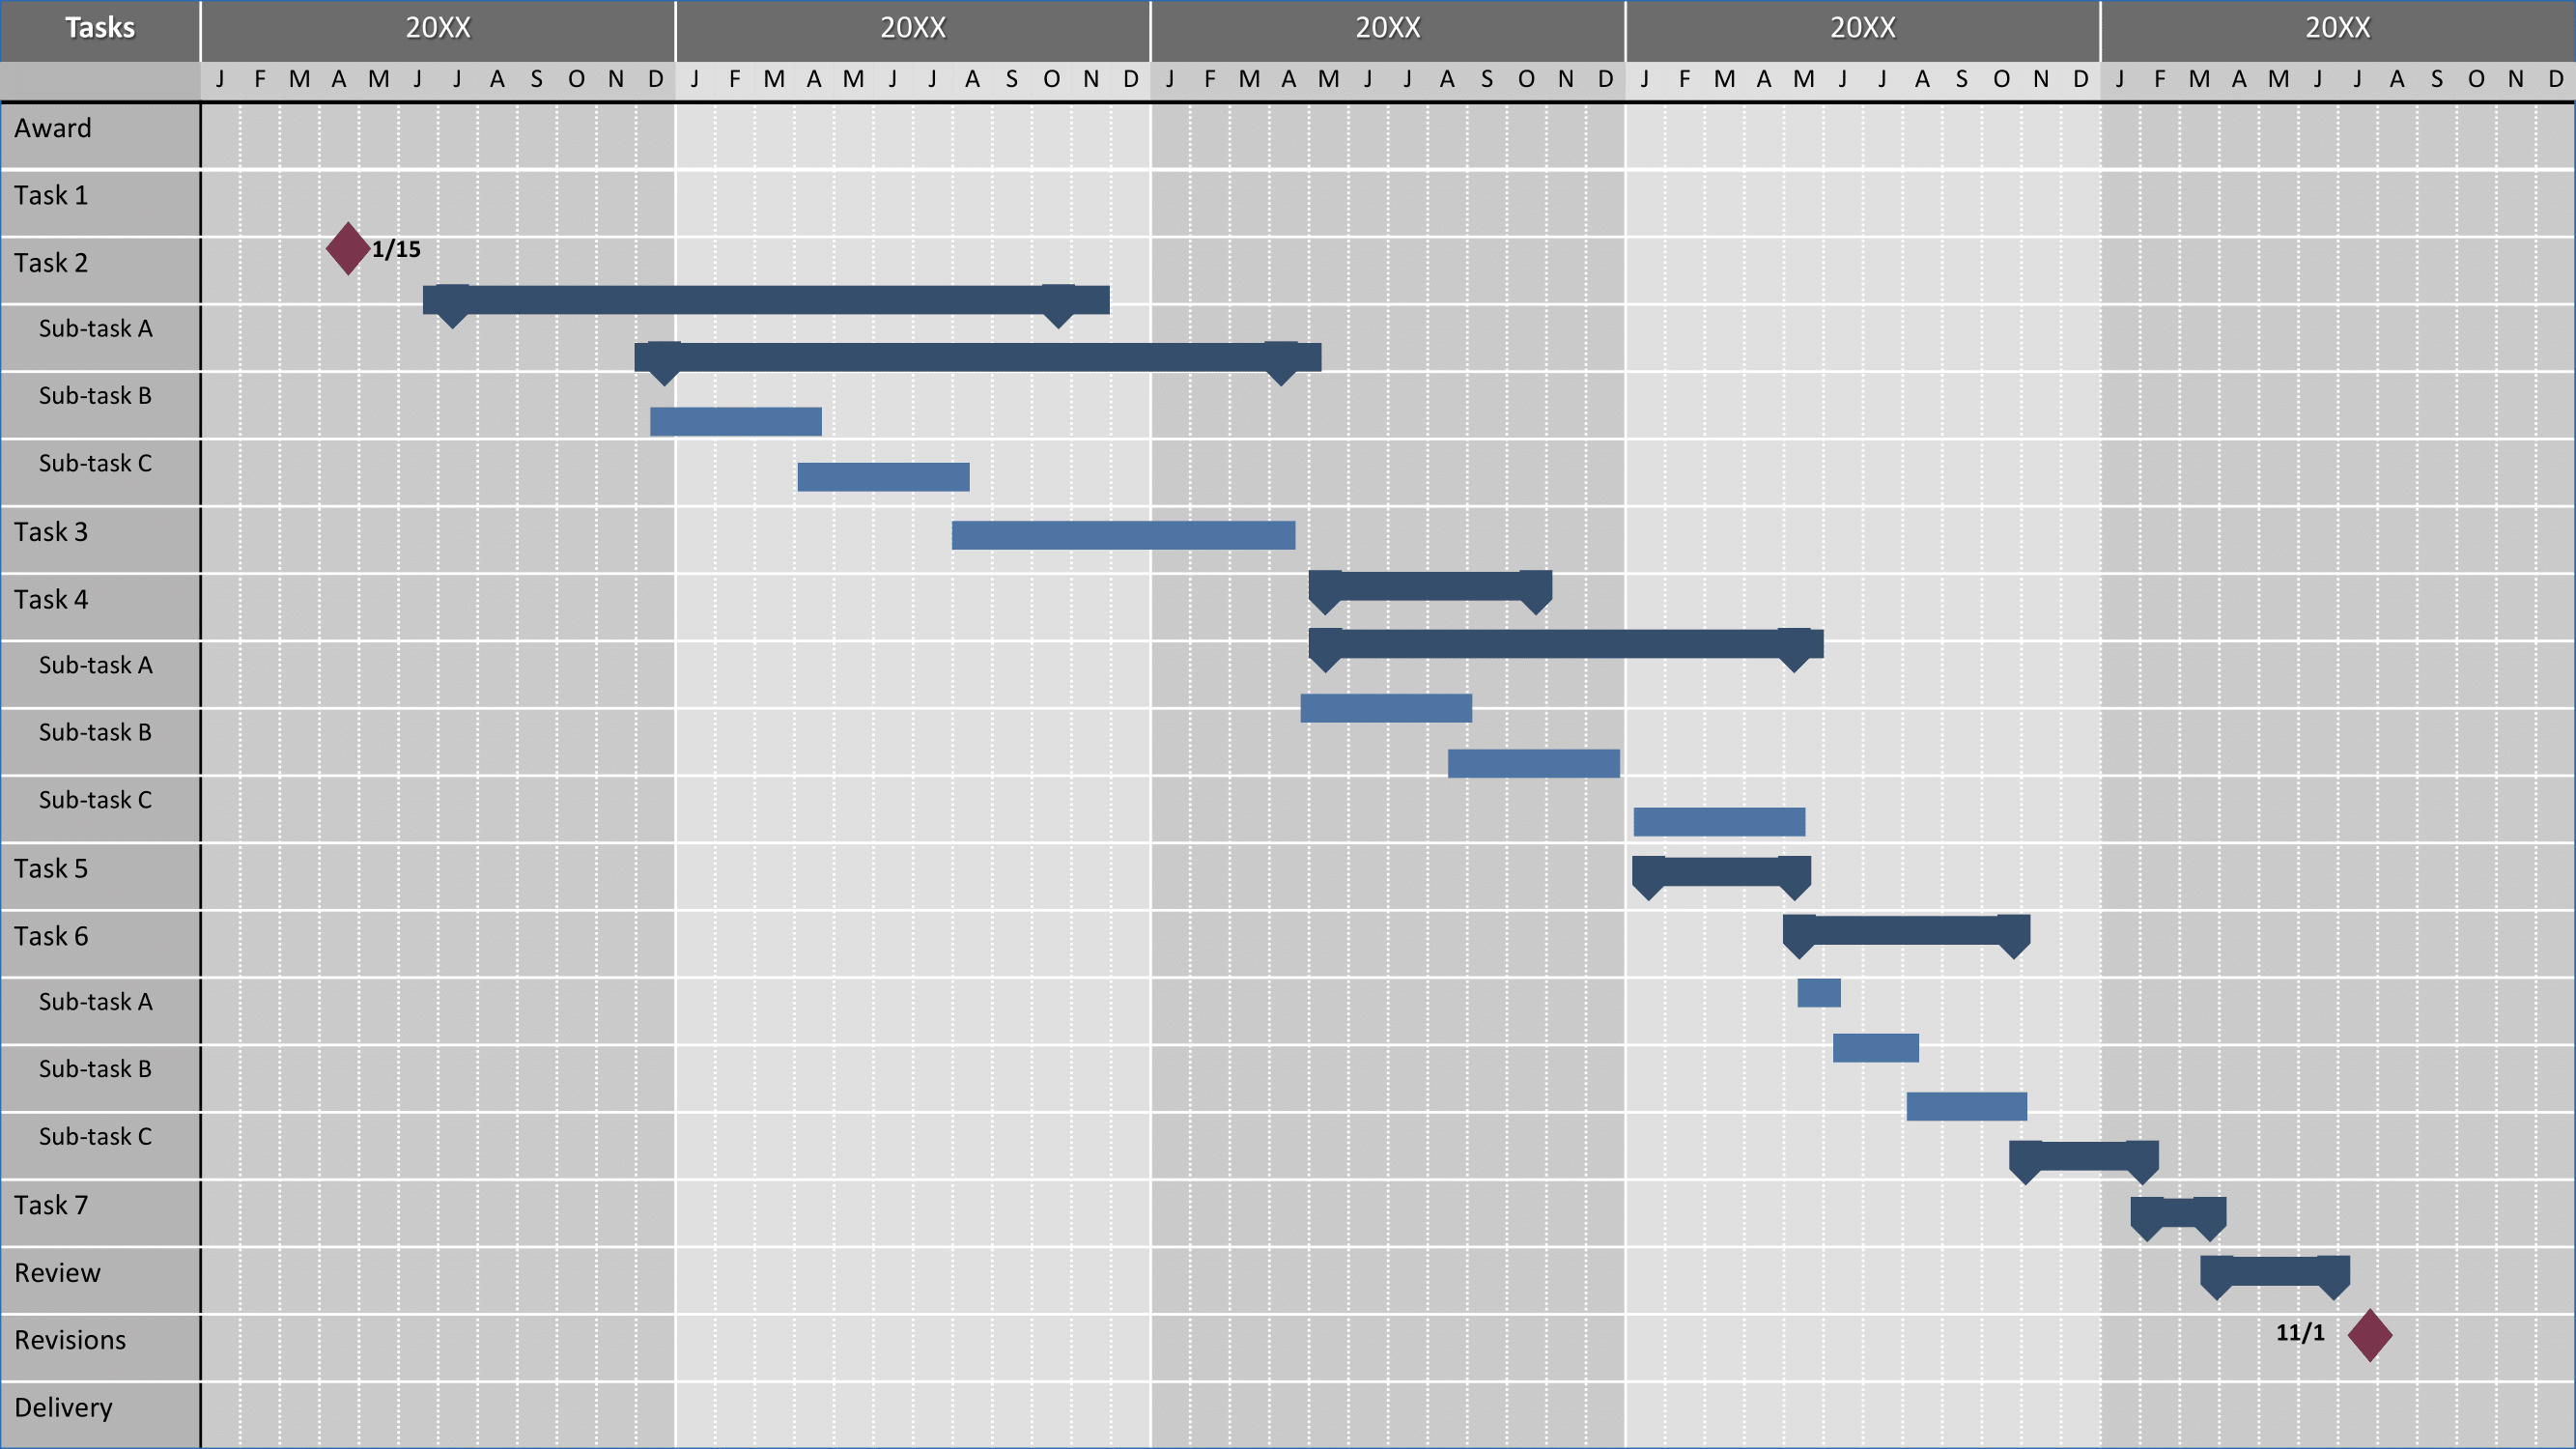
\includegraphics[scale=0.67]{../figures/gantt_template.png}
 %    }
 %    \caption{Gantt chart of the PhD project.}
 %    \label{fig:gantt}
 %    \end{figure}
 %    \end{landscape}
    

 		
% 	\newpage
% 	\section{Collaborations}
% 	\vspace*{1 cm}
%     \noindent \textbf{University - Department}\\
    
%     \noindent University address\\

% \textbf{Theme}

%     Person 1 - \href{mailto:<email>}{$<$email$>$} \\ \vspace*{-5.5mm}
    
%     Person 2 – \href{mailto:<email>}{$<$email$>$} \\

% \textbf{Theme 2}

%     Person 1 - \href{mailto:<email>}{$<$email$>$} \\ \vspace*{-5.5mm}

%     Person 2 – \href{mailto:<email>}{$<$email$>$} \\\\ 
   
    
% 	\section{Data management plan}
	
% 	\newpage
% 	% references
	\addcontentsline{toc}{section}{References}
	\bibliography{references.bib}

 %\printbibliography
	
\end{document}